
併發程序的開發通常挺難的,編寫同時需要正確和高效(換句話說,所有這些都需要)的併發程序要困難得多。對於具有許多互斥對象或無鎖的複雜性,會讓編程更加困難。

管理這種複雜性的唯一方法就是進行封裝,放入定義良好的代碼或模塊中。只要接口和需求是明確的,這些模塊的使用者就不需要知道實現是無鎖的還是基於鎖的。它確實會影響性能,所以在優化之前,模塊對於特定的需求可能不夠用,但可以根據需要進行優化,而且這些優化僅限於特定的模塊。

本章中將重點討論為併發編程實現數據結構的模塊。為什麼是數據結構,而不是算法?首先,有很多關於併發算法的文獻。其次,大多數開發者在處理算法上都有更寬裕的時間。分析代碼,相應函數花費了過多的時間,再找到了一種不同的方法來實現算法,並在性能圖表上移動到下一個高度。然後,最終會得到一個程序,其中沒有一個單獨的計算需要花費大量的時間,但仍然會有沒有達到應有速度的感覺。原因:當沒有熱代碼時,就可能有熱數據。

數據結構在併發程序中扮演著更重要的角色,因為它們決定了如何保證算法的正確性,有哪些限制,和哪些併發操作可以安全執行?不同線程看到的數據視圖是否一致?如果不知道這些問題的答案,就無法編寫代碼,而答案是由數據結構決定的。

與此同時,設計決策,比如接口和模塊邊界的選擇,會對編寫併發程序時的選擇產生重大影響,併發不能作為事後的想法添加到設計中。在設計初始,就必須考慮到併發性,特別是數據的組織。

這裡通過定義一些基本的術語和概念開始探索併發數據結構。

\subsubsubsection{6.4.1\hspace{0.2cm}併發數據結構的基礎}

使用多線程的併發程序需要線程安全的數據結構。什麼是線程安全?怎麼使數據結構是線程安全的?乍一看,似乎很簡單:如果一個數據結構可以被多個線程同時使用,並且沒有任何數據競爭(在線程之間共享),那麼它就是線程安全的。

然而,這個定義過於簡單:

\begin{itemize}
\item 將標準定的很高——例如,沒有一個STL容器是線程安全的。
\item 具有非常高的性能開銷。
\item 這通常是不必要的,開銷也是如此。
\item 在許多情況下完全沒用。
\end{itemize}

我們將逐一解決這些問題。為什麼線程安全的數據結構即使在多線程程序中也是不必要的?一種微小的可能性是,用於程序的單線程部分。我們努力最小化這些部分,因為它們對總體運行時間具有負面影響(還記得Amdahl定律嗎?),但是大多數程序都有一些需要單線程處理的事情,使這些代碼更快的方法是隻做必要的事情。更常見的不需要線程安全的情況是,即使是在多線程程序中,一個對象僅由一個線程使用。這非常常見,也是非常可取的,共享數據是併發程序中效率低下的主要原因,因此可以嘗試在每個線程上只使用本地對象和數據,獨立地完成儘可能多的工作。

但是,即使每個對象永遠不會在線程之間共享,能確定在多線程程序中使用一個類或一個數據結構是安全的嗎?這還真不一定。僅在接口層沒有看到共享,並不意味著在實現層沒有。多個對象可以在內部共享相同的數據,靜態成員和內存分配器只是其中的可能(我們傾向於認為所有需要內存的對象都通過調用\texttt{malloc()}獲得,並且\texttt{malloc()}是線程安全的,而且類也可以實現自己的分配器)。

另一方面,只要沒有線程修改對象,在多線程代碼中使用許多數據結構是安全的。但必須再次考慮實現,接口可以是隻讀的,但實現仍然是可以修改對象。如果認為這是一種奇異的可能性,請考慮標準的C++共享指針\texttt{std::shared\_ptr}。當複製一個共享指針時,複製的對象不會修改,至少不會可見(通過\texttt{const}引用傳遞給新指針的構造函數)。與此同時,知道對象中的引用計數必須增加,這意味著複製的對象已經改變(在此場景中,共享指針是線程安全的,但這不是偶然,也不是免費的,同樣也有性能成本)。

這裡需要一個更細緻的線程安全定義。但對於這個普遍的概念,沒有通用的標準,不過有幾個流行的版本。線程安全的最高級別通常稱為\textbf{強線程安全保證},提供這種保證的對象可以被多個線程併發使用,而不會引起數據競爭或其他未定義的行為(特別是,任何不變量都會保留)。下一級稱為\textbf{弱線程安全保證},只要所有線程都限制為只讀訪問(調用類的\texttt{const}成員函數),提供這種對象就可以使用多個線程同時訪問。其次,任何對對象具有獨佔訪問權的線程都可以對對象執行其他的操作(無論其他線程在同一時間做什麼)。不提供任何此類保證的對象,不能在多線程程序中使用。即使對象本身不共享,其實現內部的某些內容也很容易被其他線程修改。

本書中,將使用強弱線程安全的語言保證。提供強擔保的類有時簡單地稱為\textbf{線程安全}。只提供弱保證,則稱為\textbf{線程兼容}。大多數STL容器都提供了這樣的保證,若容器是一個線程的局部對象,可以以有效的方式使用,但若容器對象是共享的,只能調用\texttt{const}成員函數。最後,根本不提供任何保證的類稱為\textbf{線程敵對},並且不能在多線程程序中使用。

實踐中,經常遇到強保證和弱保證的組合。接口的一個子集提供強保證,其餘部分只提供弱保證。

為什麼不嘗試在設計每個對象時都有強線程安全保證呢?第一個原因是,會有性能開銷。保證通常是不必要的,因為對象不是在線程之間共享的,編寫高效程序的關鍵是不做無用的工作。更有趣的反對意見是,即使在以需要線程安全的方式共享對象,強線程安全保證可能沒用。假如需要開發一款玩家招募軍隊並進行戰鬥的遊戲。軍隊中所有單位的名稱都存儲在一個容器中,比如一個字符串列表。另一個容器存儲每個單元的當前強度。在戰役中,單位總是會被殺死或招募,遊戲引擎是多線程的,需要有效地管理龐大的軍隊。雖然STL容器只提供弱線程安全保證,但假設有一個強線程安全容器庫。這是不夠的,添加一個單元需要將它的名稱插入到一個容器中,並將初始強度插入到另一個容器中,這兩個操作本身都是線程安全的。一個線程創建一個新單元並將其插入到第一個容器中。在這個線程可以添加它的強度值之前,另一個線程看到這個新單位並需要查找它的強度,但是在第二個容器中還沒有任何東西。問題在於線程安全的保證是在錯誤的層面上提供的。從應用程序的角度來看,創建新單元是一個事務,所有遊戲引擎線程都應該能夠在添加單元之前或之後查看數據庫,但不能在中間狀態。可以通過使用互斥鎖來實現,在單元添加前鎖定,只有在兩個容器都新之後才會解鎖。在這個場景中,只要這些對象的所有訪問都由互斥鎖保護,就不用關心單個容器提供的線程安全保證。顯然,這裡需要的是一個單元數據庫,其本身提供所需的線程安全保證,例如:通過使用互斥對象。這個數據庫可能在內部使用幾個容器對象,數據庫的實現可能需要或不需要這些容器的線程安全保證,但這對數據庫的使用者應該是不可見的(擁有線程安全的容器可能會使實現更容易,也可能不會)。

這讓我們得出一個非常重要的結論:線程安全始於設計階段。必須明智地選擇程序使用的數據結構和接口,以便表示適當的抽象級別,以及發生線程交互級別上的正確事務。

考慮到這一點,本章的其餘部分應該從兩個方面來看:一方面,展示如何設計和實現一些基本的線程安全的數據結構,這些數據結構可以用在程序中,構建更復雜(和更多樣化)的構建塊。另一方面,還展示了構建線程安全類的基本技術,這些類可用於設計更復雜的數據結構。

\subsubsubsection{6.4.2\hspace{0.2cm}計數器和累加器}

最簡單的線程安全對象是簡單的計數器或累加器,計數器只是計算在線程上可能發生的一些事件。所有線程都可能需要修改計數器或訪問當前值,因此存在競爭條件。

弱線程安全保證無法滿足我們的要求,這裡需要強線程安全保證,從而確保讀取沒有更改的值總是線程安全的。我們已經看到了實現的可用選項:某種鎖、原子操作(當有原子操作時)或無鎖CAS循環。

鎖的性能因實現的不同而不同,通常首選自旋鎖。沒有立即訪問計數器的線程的等待時間將非常短,因此將線程置於睡眠狀態,並在稍後將其喚醒所需的成本根本沒有必要。另一方面,由於忙等待(輪詢自旋鎖)而浪費的CPU時間可以忽略不計,很可能只需要幾條指令。

原子指令提供了良好的性能,但操作的選擇相當有限。在C++中,可以原子地對整數進行加法,但不能對整數進行乘法。這對於簡單的計數器來說已經足夠了,但是對於累加器來說可能還不夠(累加操作可能有多個結果)。如果有一種方法可用,肯定沒有原子操作那麼簡單。

CAS循環可用於實現累加器,而不考慮需要使用的操作。然而,在大多數現代硬件上,性能比自旋鎖的性能更好(參見圖6.2),但不是最快的選擇。

當使用自旋鎖訪問單個變量或單個對象時,可以進一步優化自旋鎖。可以讓鎖成為保護對象的唯一引用,而不是通用標誌。原子變量是指針,而不是整數。除此之外,鎖定機制保持不變。因為\texttt{lock()}函數返回指向計數器的指針,所以是非標準的:

\hspace*{\fill} \\ %插入空行
\noindent
\textbf{01d\_ptrlock\_count.C}
\begin{lstlisting}[style=styleCXX]
template <typename T>
class PtrSpinlock {
	public:
	explicit PtrSpinlock(T* p) : p_(p) {}
	T* lock() {
		while (!(saved_p_ =
		p_.exchange(nullptr, std::memory_order_acquire))) {}
	}
	void unlock() {
		p_.store(saved_p_, std::memory_order_release);
	}
	private:
	std::atomic<T*> p_;
	T* saved_p_ = nullptr;
};
\end{lstlisting}

與之前的自旋鎖實現相比,原子變量的含義“顛倒”了。如果原子變量\texttt{p\_}不為空,則該鎖可用,否則為空。為自旋鎖做的所有優化在這裡也適用,看起來完全相同,所以不打算重複。另外,這個類需要一組刪除複製的操作(鎖是不可複製的)。如果需要轉移鎖,並將其釋放給另一個對象,則該鎖可以移動。如果鎖擁有它所指向的對象,析構函數應該刪除它(這結合了自旋鎖和單類中unique指針的功能)。

指針自旋鎖的第一個優點,提供了訪問保護對象的唯一方式。這就不可能有條件競爭,並在沒有鎖的情況下訪問共享數據。第二個優點,鎖的性能通常略優於常規自旋鎖,自旋鎖是否優於原子操作也取決於硬件。相同的基準測試在不同的處理器上會出現不同的結果:

%\hspace*{\fill} \\ %插入空行
\begin{center}
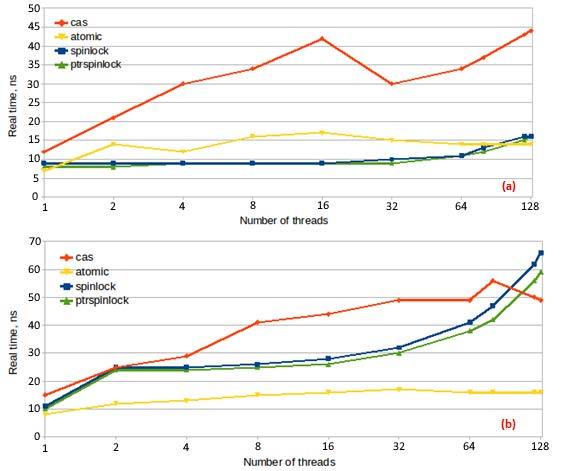
\includegraphics[width=0.9\textwidth]{content/2/chapter6/images/3.jpg}\\
圖6.3 - 共享計數增量的性能:不同硬件系統(a)和(b)的常規自旋鎖、指針自旋鎖、無鎖(比較-交換,或CAS)和無等待(原子)
\end{center}

通常,越新的處理器處理鎖和忙等待的性能越好,而且自旋鎖在最新的硬件上提供的性能也越好(圖6.3中,系統\textit{b}使用的Intel x86 CPU比系統\textit{a}的CPU晚一代)。

執行一個操作所需的平均時間(或者相反的,吞吐量)是我們在大多數HPC系統中主要關注的指標。然而,這並不是用來衡量併發程序性能的唯一指標。如果程序在移動設備上運行,那麼功耗可能更重要。所有線程使用的CPU總時間根據平均功耗的進行調整。用於測試計數器增量平均實時時間的基準測試,同樣也可以用來測試CPU時間:

%\hspace*{\fill} \\ %插入空行
\begin{center}
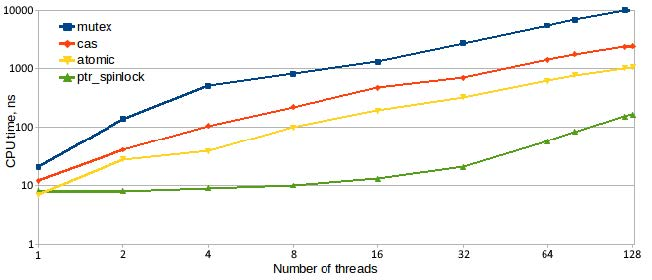
\includegraphics[width=0.9\textwidth]{content/2/chapter6/images/4.jpg}\\
圖6.4 - 線程安全的計數器——不同實現使用的平均CPU時間
\end{center}

壞消息是,無論採用哪種實現,多個線程同時訪問共享數據的成本都會隨著線程數量的增加呈指數增長,至少在有很多線程的情況下是這樣的(注意,圖6.4中的y軸比例是對數的)。然而,不同的實現之間的效率差別很大,對於最高效的實現來說,在8個線程之後才會出現指數級的增長。注意,不同硬件系統的結果也會有所不同,所以必須根據目標平臺進行選擇,並且只有在完成測試後才能選擇。

無論選擇何種實現,線程安全的累加器或計數器都不應將其公開,而應將其封裝在類中。原因之一是為類的客戶端提供穩定的接口,同時保留優化實現的自由度。

第二個原因更微妙,與計數器提供的保證有關。目前,關注的是計數器本身,確保所有線程都可以對其進行修改和訪問,而不存在任何競爭。這是否足夠使用,取決於如何使用計數器。如果只是計算一些不依賴於計數器的值,那麼只關心值本身是否正確就好。另一方面,如果計數的是數組中的元素數量,那麼處理的就是數據依賴關係。假設有一個大型的預分配數組(或者一個容器,可以在不影響現有元素的情況下增長),所有線程都在計算要插入到這個數組中的新元素。計數器對進行計算的元素進行計數,並將值插入數組,可以由其他線程使用。若一個線程從計數器中讀取值N,必須確保數組的前N個元素可以安全讀取(這意味著沒有其他線程修改它們)。但是數組本身既不是原子的,也不受鎖的保護。可以通過鎖來保護對整個數組的訪問,但這可能會降低程序的性能。如果數組中已經有很多元素了,只有一個線程可以讀取它們,那麼程序就可能是單線程的。另一方面,從多個線程讀取常量、不可變數據都是安全的,不需要任何鎖。只需要知道不可變數據和變化數據之間的邊界在哪裡,而這正是計數器應該提供的。這裡的關鍵問題是內存可見性,需要在計數器的值從N-1更改為N之前,保證數組前N個元素的更改對所有線程都可見。

上一章中,瞭解控制可見性的方法是通過限制內存序或使用內存柵欄(同一件事的兩種不同的方式)。在多線程程序中,計數和索引的區別在於,索引提供了額外的保證。如果將索引從N-1增加到N的線程在增加索引之前已經完成了數組元素N的初始化,然後其他線程讀取索引並獲得N(或更大)的值,保證至少有N個元素完全初始化,並且可以安全地讀取數組中的元素(假設沒有其他線程寫入這些元素)。這個保證很重要,多個線程正在訪問內存中的相同位置(數組元素N)而沒有任何鎖,其中一個線程正在寫入這個位置,訪問是安全的,沒有數據競爭。若不能使用共享索引來確認這種保證,則需要鎖定對數組的所有訪問,並且只有一個線程能夠讀取它。可以使用這個原子索引類:

\hspace*{\fill} \\ %插入空行
\noindent
\textbf{02\_atomic\_index.C}
\begin{lstlisting}[style=styleCXX]
class AtomicIndex {
	std::atomic<unsigned long> c_;
	public:
	unsigned long incr() noexcept {
		return 1 + c_.fetch_add(1, std::memory_order_release);
	}
	unsigned long get() const noexcept {
		return c_.load(std::memory_order_acquire);
	}
};
\end{lstlisting}

唯一不同的是,索引在計數是在內存可見性保證,而計數不提供這種可見性保證:

\begin{lstlisting}[style=styleCXX]
class AtomicCount {
	std::atomic<unsigned long> c_;
	public:
	unsigned long incr() noexcept {
		return 1 + c_.fetch_add(1, std::memory_order_relaxed);
	}
	unsigned long get() const noexcept {
		return c_.load(std::memory_order_relaxed);
	}
};
\end{lstlisting}

當然,每個類的線程安全和內存可見性保證都應該有相應的文檔,兩者之間是否存在性能差異取決於硬件。而在x86 CPU上沒有區別,因為是請求還是不請求,用於原子增量和原子讀取的硬件指令都有“類索引”的內存柵欄存在。在ARM CPU上,自由(或無障礙)內存操作明顯更快。但是,不管性能、清晰度和問題是什麼,都不應該忘記:如果開發者使用一個索引類,其會顯式地提供了內存序保證,但沒有索引任何東西。每個讀者都會想知道發生了什麼,以及使用這些保證的代碼中技巧和位置在哪裡。通過正確的文檔保證集的接口,就可以向讀者表明編寫這段代碼的意圖了。

現在回到本節中的“隱藏”成就。我們學習了線程安全的計數器,但在此過程中,提出了一種算法,似乎違反了編寫多線程代碼的第一條規則:任何時候兩個或多個線程訪問相同的內存位置,訪問必須帶鎖(或原子的)。沒有鎖定共享數組,允許在其元素中包含任意數據(所以它可能不是原子的),而且還成功了!用來避免數據競爭的方法是為併發設計的數據結構的基礎,現在再花些時間更好地理解和概括它。

\subsubsubsection{6.4.3\hspace{0.2cm}發佈協議}

我們試圖解決的問題是,在數據結構設計和併發程序開發中非常常見的問題。線程正在創建新數據,程序的其餘部分只能夠在數據準備好時看到這些數據。創建數據的線程通常稱為寫線程或生產者線程,其他線程都是讀取線程或消費者線程。

最簡單的解決方案是使用鎖,並嚴格遵守避免數據競爭的規則。如果多個線程(檢查)必須訪問相同的內存位置(檢查),並且至少有一個線程在這個位置進行寫操作(我們的例子中正好是一個線程——檢查),那麼所有線程在訪問這個內存位置進行讀寫操作之前都必須獲得鎖。這種解決方案的缺點在於性能,生產者在完成並且不再發生寫操作之後很長一段時間,所有的消費者線程都會互相鎖定,從而不能併發地讀取數據。現在,只讀訪問根本不需要鎖,但需要在程序中有一個保證點,這樣所有的寫操作都發生在這一點之前,所有的讀操作都發生在這一點之後。所有的使用者線程都在只讀環境中操作,不需要任何鎖。挑戰在於保證讀寫之間的邊界,除非進行了某種同步,否則內存的可見性是不能保證的。因為寫入器已經完成了對內存的修改,並不意味著讀取器可以看到內存的最終狀態。鎖包括相應的內存柵欄,它們為臨界區設置邊界,並確保在臨界區之後執行的操作都將看到在臨界區之前或期間發生的所有內存更改。但現在我們想在沒有鎖的情況下,獲得同樣的保證。

這個問題的無鎖解決方案依賴於非常特殊的協議,從而可以在生產者和消費者線程之間傳遞信息:

\begin{itemize}
\item 
生產者線程在內存中準備時,其他線程無法訪問的數據。可以由生產者線程分配的內存,也可以是預分配的內存。這裡,生產者是唯一對該內存有有效引用的線程,而該有效引用不會與其他線程共享(可能其他線程有訪問該內存的方法,但這將引起程序的錯誤,類似於索引數組超出邊界)。因為只有一個線程訪問新數據,所以不需要同步。至於其他線程,這些數據根本看不到。

\item 
所有的消費者線程都必須使用共享指針來訪問數據,稱之為\textit{根指針},這個指針最初是空的。在生產線程構造數據時,它保持為空。所以,從消費者線程的角度來看,目前沒有數據。更一般地說,“指針”不需要是一個實際的指針:任何類型的句柄或引用都可以用,只要是允許訪問內存位置,並且可以設置為一個無效值。如果所有的新對象都是在預先分配的數組中創建的,那麼“指針”可以是數組的索引,無效值可以是大於或等於數組長度的值。

\item 
協議的關鍵在於,消費者訪問數據的唯一方式是通過\textit{根指針},在生產者準備顯示或發佈數據之前,根指針保持為空。發佈數據的過程非常簡單,生產者必須在根指針中存儲數據的正確內存位置,並且這個改變必須伴隨著內存釋放柵欄。

\item 
消費者可以以原子方式再次查詢根指針。如果查詢返回空,則沒有數據(就使用者而言),使用者線程應該等待,或者做一些其他的工作。如果查詢返回一個非空值,那麼數據就準備好了,生產者將不再更改它。該查詢必須與獲取內存柵欄一起完成,它與生產者端的釋放內存柵欄一起,確保在觀察到指針值的變化時,新數據是可見的。
\end{itemize}

這個過程有時稱為\textbf{發佈協議},因為它允許生產者線程以一種保證沒有數據競爭的方式發佈信息,供其他線程使用。發佈協議可以使用允許訪問內存的句柄來實現,只要這個句柄可以進行原子性修改。當然,指針是最常用的句柄,後面是數組下標。

發佈的數據可以是簡單的,也可以是複雜的,這都無所謂。甚至不必是單個對象或單個內存位置,\textit{根指針}所指向的對象本身可以包含指向多個數據的指針。發佈協議的關鍵點為:

\begin{itemize}
\item
所有消費者都通過\textit{根指針}訪問一組特定的數據。訪問數據的唯一方法是讀取\textit{根指針}的非空值。

\item
生產者可以以任何方式準備數據,這是\textit{根指針}仍然是空的。生產者可以對線程本地的數據進行引用。

\item 
當生產者想要發佈數據時,會自動設置\textit{根指針}指向正確的地址,並釋放柵欄。數據發佈後,生產者不能改變它(其他線程也不能)。

\item 
消費者線程必須以原子的方式讀取\textit{根指針},並獲取柵欄。如果讀取非空值,則可以通過\textit{根指針}讀取可訪問的數據。

\end{itemize}

當然,用於實現發佈協議的原子讀寫不應該分散在代碼中,應該實現一個發佈指針類來封裝這個功能。下一節中,我們將看到這個類的一個簡單實現。

\subsubsubsection{6.4.4\hspace{0.2cm}併發編程的智能指針}

併發(線程安全)數據結構的挑戰是,如何以線程安全的方式添加、刪除和更改數據。發佈協議提供了一種向所有線程發佈新數據的方法,它通常是向任何此類數據結構添加新數據的第一步。因此,首先來瞭解如何將協議的指針封裝入類。

\hspace*{\fill} \\ %插入空行
\noindent
\textbf{發佈指針}

下面是一個發佈指針,包含了\texttt{unique\_ptr}(或擁有指針)的功能(所以可以稱它為線程安全的\texttt{unique\_ptr}):

\hspace*{\fill} \\ %插入空行
\noindent
\textbf{03\_owning\_ptr\_mbm.C}
\begin{lstlisting}[style=styleCXX]
template <typename T>
class ts_unique_ptr {
	public:
	ts_unique_ptr() = default;
	explicit ts_unique_ptr(T* p) : p_(p) {}
	ts_unique_ptr(const ts_unique_ptr&) = delete;
	ts_unique_ptr& operator=(const ts_unique_ptr&) = delete;
	~ts_unique_ptr() {
		delete p_.load(std::memory_order_relaxed);
	}
	void publish(T* p) noexcept {
		p_.store(p, std::memory_order_release);
	}
	const T* get() const noexcept {
		return p_.load(std::memory_order_acquire);
	}
	const T& operator*() const noexcept { return *this->get(); }
	ts_unique_ptr& operator=(T* p) noexcept {
		this->publish(p); return *this;
	}
	private:
	std::atomic<T*> p_ { nullptr };
};
\end{lstlisting}

當然,這是一個非常簡單的設計。完整的實現應該支持一個自定義刪除器,移動構造函數和賦值操作符,也許還有很多特性,類似於\texttt{std::unique\_ptr}。標準不保證訪問存儲在\texttt{std::unique\_ptr}對象中的指針值是原子的,或者使用了必要的內存柵欄,所以\texttt{std::unique\_ptr}不能用來實現發佈協議。

現在,應該清楚線程安全的\texttt{unique\_ptr}提供了什麼。關鍵函數是\texttt{publish()}和\texttt{get()},它們實現了發佈協議。注意,\texttt{publish()}方法不會刪除舊數據,假設生產者線程只調用一次\texttt{publish()},並且只調用一個空指針。可以為此添加一個斷言,在調試版本中這樣做可能是一個好主意,但也關心性能問題。說到性能,基準測試顯示,對發佈指針進行單線程解引用的時間與原始指針或\texttt{std::unique\_ptr}的解引用時間相同。基準測試也並不複雜:

\begin{lstlisting}[style=styleCXX]
struct A { … arbitrary object for testing … };
ts_unique_ptr<A> p(new A(…));
void BM_ptr_deref(benchmark::State& state) {
	A x;
	for (auto _ : state) {
		benchmark::DoNotOptimize(x = *p);
	}
	state.SetItemsProcessed(state.iterations());
}
BENCHMARK(BM_ptr_deref)->Threads(1)->UseRealTime();
… repeat for desired number of threads …
BENCHMARK_MAIN();
\end{lstlisting}

運行這個基準測試可以瞭解對無鎖發佈指針的解引用有多快:

%\hspace*{\fill} \\ %插入空行
\begin{center}
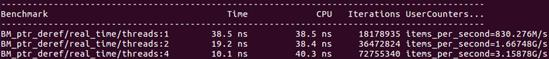
\includegraphics[width=0.9\textwidth]{content/2/chapter6/images/5.jpg}\\
圖6.5 - 發佈指針(消費者線程)的性能
\end{center}

結果應該與對原始指針的解引用進行比較,在多線程中也可以這樣做:

%\hspace*{\fill} \\ %插入空行
\begin{center}
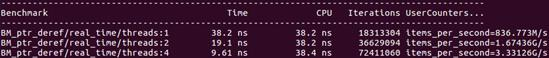
\includegraphics[width=0.9\textwidth]{content/2/chapter6/images/6.jpg}\\
圖6.6 - 原始指針的性能,與圖6.5進行比較
\end{center}

性能數據非常接近。還可以比較發佈的速度,但消費者端更重要。每個對象只發布一次,然後進行多次訪問。

瞭解發佈指針不做什麼同樣重要。首先,在指針的構造中沒有線程安全問題。假設生產者和消費者線程共享對構造好的指針,這個指針初始化為空。誰來構造並初始化了指針?在數據結構中,都有一個\textit{根指針},通過它可以訪問整個數據結構,它由構造初始數據結構的線程初始化。還有一些指針,可作為某些數據元素的根,本身包含在另一個數據元素中。現在,想象一個簡單的單鏈表,其中每個元素的“next”指針是下一個元素的根,而頭是整個鏈表的根。生成鏈表元素的線程必須將“next”指針初始化為空。然後,另一個生產者可以添加一個新元素併發布。注意,這偏離了數據發佈後就不可變的規則。但是,這裡可以這樣做,因為對線程安全\texttt{unique\_ptr}的更改都是原子的。無論如何,沒有線程可以在指針構造的時候進行訪問非常關鍵(這是一個非常常見的限制,大多數構造都不是線程安全的,因為對象在構造之前不存在,所以不能保證)。

指針沒有做的事是,沒有為多個生產者線程提供同步。如果兩個線程試圖通過同一個指針發佈新數據,結果是未定義的,並且存在數據競爭(一些消費者線程將看到一組數據,而其他線程將看到不同的數據)。如果有多個生產者線程操作特定的數據結構,必須使用一種機制進行同步。

最後,雖然指針實現了線程安全的發佈協議,但沒有執行安全的“取消發佈”和刪除數據。它是擁有指針的,因此當刪除時,所指向的數據也會刪除。但消費者線程可以使用刪除之前獲得的值。數據所有權和生命週期的問題都必須處理。理想情況下,程序中應該有一個點,在這個點上,知道整個數據結構或不再需要某個子集了。消費者線程都不應該訪問這些數據,甚至不應該保留指向它的指針。此時,\textit{根指針}和其指向的內容就可以安全的刪除例如。在執行過程中如何安排,就是是另外一件事情了,通常由算法控制。

有時,希望指針能夠以線程安全的方式同時管理數據的創建和刪除。本例中,我們需要一個線程安全的共享指針。

\hspace*{\fill} \\ %插入空行
\noindent
\textbf{原子共享指針}

如果不能保證程序中有已知的點可以安全地刪除數據,就必須清楚有多少消費者線程持有有效的數據指針。如果想要刪除這個數據,必須等到在整個程序中只有一個指針指向它時,再安全地刪除數據和指針本身(或至少將其重置為空)。這是進行引用計數共享指針的工作模式,計算有多少指向同一對象的指針,在沒有對該指針的引用時,將該指針刪除。

討論線程安全的共享指針時,理解指針需要什麼保證非常重要。C++標準共享指針\texttt{std::shared\_ptr}通常是線程安全的。如果多個線程操作指向同一對象的不同共享指針,那麼對引用計數器的操作是線程安全的,即使兩個線程導致計數器同時改變。若一個線程正在複製它的共享指針,而另一個線程正在刪除它的共享指針,並且在這些操作開始之前引用計數是N,計數器將上升到N+1,然後回到N(或先下降,然後上升,中間值可以是N+1或N-1,但不存在數據競爭,並且行為很明確,包括最終狀態。這個保證意味著引用計數器上的操作是原子的。實際上,引用計數器是一個原子整數,實現時使用\texttt{fetch\_add()}對其進行原子遞增或遞減。

只要沒有多個線程共享同一個共享指針,這個保證就適用。如何獲得每個線程自己的共享指針是另外一個問題,因為所有指向同一對象的共享指針必須以第一個指針的方式進行創建,這些指針必須在某個時間點從一個線程傳遞到另一個線程。假設,複製共享指針的代碼受到互斥鎖的保護。如果兩個線程訪問同一個共享指針,那麼所有的猜測都是多餘的。若一個線程試圖複製共享指針,同時另一個線程正在重置它,結果是未定義的。特別是,標準共享指針不能用於發佈協議的實現。然而,當共享指針的副本分發到線程(可能處於鎖定狀態)中,共享的所有權就會得到保護,對象的刪除將以線程安全的方式處理。當最後一個指向該對象的共享指針刪除時,該對象也會刪除。請注意,由於每個特定的共享指針都會由一個線程處理,所以這是完全安全的。如果在程序執行期間,只有一個共享指針擁有對象時,那麼也只有一個線程可以訪問這個對象。其他線程不能複製這個指針(不讓兩個線程共享同一個指針對象),並且沒有其他方法可以獲得指向同一個對象的指針,所以刪除操作將以單線程的方式進行。

這種方式很好,但兩個線程會訪問同一個共享指針呢?這種訪問的例子就是發佈協議。消費者線程正在讀取指針的值,而生產者線程可能正在修改它,這樣就需要共享指針本身的操作是原子的。在C++20中可以這樣做,這裡允許寫\texttt{std::atomic<std::shared\_ptr<T>>}。注意,早期的建議寫一個新類代替\texttt{std::atomic\_shared\_ptr<T>}。不過,這也不是最終的方法。

如果沒有兼容C++20的編譯器和相應的標準庫,或者不能在代碼中使用C++20的話,仍可以在\texttt{std::shared\_ptr}上執行原子操作,但需要顯式地做。為了使用在所有線程之間共享的指針\texttt{p\_}發佈對象,生產者線程必須這樣做:

\begin{lstlisting}[style=styleCXX]
std::shared_ptr<T> p_;
T* data = new T;
… finish initializing the data …
std::atomic_store_explicit(
	&p_, std::shared_ptr<T>(data), std::memory_order_release);
\end{lstlisting}

另一方面,為了獲得指針,消費者線程必須這樣做:

\begin{lstlisting}[style=styleCXX]
std::shared_ptr<T> p_;
const T* data = std::atomic_load_explicit(
	&p_, std::memory_order_acquire).get();
\end{lstlisting}

與C++20原子共享指針相比,這種方法的主要缺點是無法避免非原子訪問。開發者應該記住始終使用原子函數來操作共享指針。

雖然方便,但\texttt{std::shared\_ptr}並不是一個特別有效的指針,並且原子訪問使它變得很慢。可以比較上一節中使用線程安全的發佈指針和使用顯式原子訪問共享指針發佈對象的速度:

%\hspace*{\fill} \\ %插入空行
\begin{center}
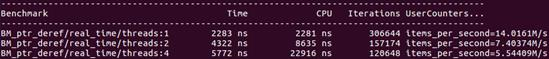
\includegraphics[width=0.9\textwidth]{content/2/chapter6/images/7.jpg}\\
圖6.7 - 原子共享發佈指針的性能(消費者線程)
\end{center}

同樣,應該將這些數字與圖6.5中的數字進行比較。發佈指針在一個線程上要快60倍,而且這種優勢會隨著線程的數量變多而增加。當然,共享指針的意義在於提供了共享資源的所有權。因此,共享指針需要更多的時間來完成更多的工作。比較的重點是顯示這種共享所有權的成本。如果可以避免,程序的效率會更高。

即使需要共享所有權(如果沒有共享所有權,有些併發數據結構很難設計),使用有限的功能和最實現設計自己的引用計數指針,則可以完成得更好,一種常見的方法是使用侵入引用計數。侵入式共享指針將其引用計數存儲在指向的對象中。當為特定對象(如特定數據結構中的列表節點)設計時,對象在設計時需要考慮到共享所有權,幷包含引用計數器。否則,可以對任何類型使用包裝器類,並使用引用計數器進行擴展:

%\hspace*{\fill} \\ %插入空行
\noindent
\textbf{04\_intr\_shared\_ptr\_mbm.C}
\begin{lstlisting}[style=styleCXX]
template <typename T> struct Wrapper {
	T object;
	Wrapper(… arguments …) : object(…) {}
	~Wrapper() = default;
	Wrapper (const Wrapper&) = delete;
	Wrapper& operator=(const Wrapper&) = delete;
	std::atomic<size_t> ref_cnt_ = 0;
	void AddRef() {
		ref_cnt_.fetch_add(1, std::memory_order_acq_rel);
	}
	bool DelRef() { return
		ref_cnt_.fetch_sub(1, std::memory_order_acq_rel) == 1;
	}
};
\end{lstlisting}

當減少引用計數時,要知道何時達到0(或在減少之前是1),共享指針就會刪除對象。

即使是最簡單的原子共享指針的實現也相當冗長,本章的示例代碼中可以找到一個非常簡單的示例。同樣,這個示例只包含指針正確執行幾個任務所需的最小值,例如:發佈對象和多個線程併發地訪問同一個指針。這個例子的目的是讓我們更容易理解實現這類指針所需的基本元素(即使這樣,代碼也有幾頁長)。

除了使用侵入式引用計數器外,特定於應用的共享指針可以放棄\texttt{std::shared\_ptr}的其他特性,例如:許多應用程序不需要弱指針。一個極簡的引用計數指針可以比標準指針高效幾倍:

%\hspace*{\fill} \\ %插入空行
\begin{center}
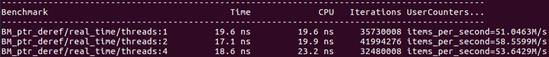
\includegraphics[width=0.9\textwidth]{content/2/chapter6/images/8.jpg}\\
圖6.8 - 自定義原子共享發佈指針(消費者線程)的性能
\end{center}

同樣,對於指針的賦值和重賦值、兩個指針的原子交換以及指針上的其他原子操作,它的效率更高。這個共享指針比唯一指針的效率低得多,若可以顯式地管理數據所有權,則不需要引用計數。

現在,我們瞭解了數據結構的兩個關鍵構建塊,可以添加新數據併發布它(向其他線程顯示),並需要跟蹤其所有權,甚至是跨線程(這需要付出巨大代價)。




















